%-----------------------------------------------------------------------------% 14.04.2026
% energy function & Herletiung, maximieren , Optimierungsalg in Anwendungen
% Zusammenhang zwischen max likelihood 
% mehr in Text einbetten, python packages um kf implementieren



% Meeting 12. Juni 2025
%------------------------------------------------------------------------------

% mit Beispiel zwei dim random walk 
% Problembeschreibung 
% Bayes -> realtime problem

%------------------------------------------------------------------------------
% Hintergrund Wahrscheinlichkeitstheorie, Bayes' rule, conditioning
% einfacheres Beispiel Zeit, Dynamik, Observation, likelihood mit Bayes -> Problem 

% Gold als Testbeispiel: Kann als einfaches Beispiel genutzt werden, später auf komplexere Sets erweitern

% Random Walk Problem:
% Mit Bayes’scher Methode theoretisch berechenbar, aber praktisch problematisch, da Komplexität mit der Zeit t wächst

% Iterative Lösung nötig, um Berechnung für jeden Zeitschritt effizient durchzuführen → Filtering Equations

% Bayesian Filtering & Kalman Filter:
% Wird eingeführt, um bewegte Objekte zu tracken (z. B. Tracking eines Objekts mit Dynamik) ==> gutes Beispiel suchen

% Beispiel: Observation mit Noise – Kalman Filter hilft, den Zustand iterativ zu schätzen

% Struktur der Arbeit:
% Zuerst Bayes’sche Methode erklären (Kapitel 2)
% Dann Kalman Filter als iterative Lösung einführen
% Beispielrechnung zeigen, um die Methode zu veranschaulichen



%------------------------------------------------------------------------------
% Meeting 17. Juni 2025
%------------------------------------------------------------------------------

% Q: replace k with t for the time steps? 
% A: YES

% q könnte v beeinflussen, würde nicht auf einer Linie fliegen
% update: geschwindigkeit und nicht Position -> durch measurement Model ungenau sehen

% Loop schreiben, t in 1:T
% x= transition update
% y= observation
% x und y abspeichern

% Matrixmultiplikation mit numpy

% random sampling, gaussian
% mit numpy machen, falls es nicht funktioniert: scipy für mehr Verteilungen .stats, interface intuitiver

%------------------------------------------------------------------------------

\textcolor{orange}{noch umformulieren}


%------------------------------------------------------------------------------
% Meeting 22. Juli 2025
%------------------------------------------------------------------------------

% energy_function muss ich nicht coden, wird schon in filterpy gemacht
% Kalman filter package benutzen

% energy_function hänge von theta ab, und theta hängt von den Daten ab
% allgemeine Rekursion machen mit filtering, Filter mit Parameter die mich interessieren initialisieren, score = 0 setzen und durch Daten iterieren und log_likelihood benutzen

% es gibt keine Methode, die die energy_function raus gibt, muss trotzdem Filter laufen lassen und extrahieren und zusammen zählen

% Funktion mit einem Argument -> numpy array sein, Teil von diese, array extrahieren um in der Funktion zu brauchen 


%------------------------------------------------------------------------------
% Meeting 19. August 2025
%------------------------------------------------------------------------------

% Random walk = a type of system model.

% Kalman filter = an algorithm that can estimate the hidden states of such a system, even when measurements are noisy.

%------------------------------------------------------------------------------
% Meeting 6. Oktober 2025
%------------------------------------------------------------------------------

% letzte Data vom Trainingssatz nehmen -> für den Anfang vom Testset
% gefiltertes nahe bei den testdaten, weil Varianz von observation noise so tief ist gefittet worden, kann es fast exakt filtern (mehr oder weniger), observation folgen dann also exakt der Kurve. D.h. Model ist genug flexibel, dass es mit der dynamischen Gleichung all die Bewegungen erklären kann. Darum wählt es einen kleinen Wert für Noise. Nehmen wir z.B. an man hätte ein weniger flexibles Model, eins wo nur sehr langsam den Kurs verändern könnte oder so. Nehmen wir an es wäre ein lineares Model, es wäre nur eine Linie. Dann müsste all die Variation von der Observation noise kommen. In diesem Fall könne wir das ganze durch einen Random Walk erklären. Fürs filtern ist es deshalb nicht so erstaunlich, dass es genau gleich ist. Filtern ist der estimate vom state nachdem ich es gesehen habe. 

% wenn ich weiss, dass ich nur observation error habe, dann ist der beste guess für den state, wenn ich observation gemacht habe es gleich observation zu setzen. darum folgt das gefilterte genau dem gemessenenem. Das heisst nicht, dass meine predictions perfekt sind, weil predictions hängen davon ab wie gut ich voraussagen kann. Darum liegen sie auch leicht falsch. Wenn die Messung genau ist, dann kann man für das gefilterte genau das nehmen, wo man beobachtet hat. 

% Intepretation: hat state gefiltert und jetzt predictet es für den nächsten state genau das gleiche, weil der process noise klein gefittet worden ist. der mse ist gross, wenn ich immer den gleichen state nehme wie den nächsten, ist der Fehler gross. 
% Ausprobieren, wenn mer grossen prozess noise nimmt, ob prediction dann random sind oder nicht. 0.2 varianz

% bei measurement tut es den noise nicht dazuzählen, darum ist es genau gleich. wenn man den nächsten Wert aus der Dynamik simulieren würde, dann hätte ich einen zufälligen noise Term dabei. 

% observation genau gleich wie state, weil H = 1 (30)

% Prediction ist $p(y_t | x_{1:t-1}) \sim y^\sim_t$ eine Verteilung

% Hier nehmen wir den Mittelwert. Prediction ist nicht sample von dieser Verteilung sondert Erwartungswert. Und weil der Random Walk symmetrisch ist, ist es der Erwartungswert gleich wie der gefilterte Wert. (nicht erwartet) wegen Kalman Filter, predicten ist immer im Mittelwert. 

% Interpretation: wenn das observed werte sind, sind beim random walk, sofern der gefilterte wert genau beim observed wert ist, dann ist der estimate für den Erwartungswert von $p(x_t |x_{1:t-1})$. das ist das gefilterte. und prediction beim random walk model ist genau das gleiche. weil wenn ich einen schritt mache, ändere ich nicht den erwartungswert. Der mittelwert bleibt genau gleich. Benutze für den nächsten wert den jetztigen state. Durch das filtern beobachte ich das und dann sage ich das wäre der richtige wert gewesen. 

% Beim trend model hat man nicht nur random walk sondern auch noch einen trend. Für prediction den jetzigen wert und den trend nehmen. Versetzt um den Trend. 

% Wie würde ich alle Zukunft vorausschauen? Im Random Walk: Prediction für Zukunft wäre eine Gerade -> genau der gleiche Wert. Erwartungswert in der Zukunft bleibt genau gleich. 
% Im Trendmodel, habe ich einen Trend estimated und bei prediction gehe ich in der Zukunft genau mit diesem Trend weiter. Bei jedem Zeitschritt passe ich den basiswert und den Trend an. Beim Random Walk model nur Basiswert anpassen. 

% prediction: mittelwert von predictive Verteilung nehmen, das macht auch Sinn, weil es der Wert ist, den der mean square error am kleinsten macht. 
% wenn ich eine Verteilung durch eine Zahl abschätzen muss, dann ist der Erwartungswert diese Zahl, wo im Schnitt den squared error am kleinsten macht. Zahl, wo das minimiert, ist 
% Erwartungswert ist die Zahl, das wenn ich über lange Zeit meine Zufallsvariable mit dieser Zahl abschätze, mache ich am wenigsten squared error. Darum macht es auch Sinn, das wenn man den Mean Squared Error von den Predictions minimieren möchte, das man den Erwartungswert nimmt von der Verteilung als prediction. das wo man im Schnitt bekommen würde. wenn man andere distanz hätte, wo man minimieren möchte, müsste man eine andere Zahl nehmen wo nicht unbedingt erwartungswert ist zb absolute error minimieren, dann ... im Fall der Normalverteilung ist es gleich

% für prediction muss man eine Zahl wählen, und man hat nur die Verteilung gegeben. Dann fasst man die Verteilung zu einer Zahl zusammen und der Erwartungswert macht hier Sinn. Weil Erwartungswert von einem Random Walk ist Null. 

% y_train sollte erste Anfangsindize sein. 

% gefilterte kovarianz ist das was das model updated. Wahl von P0 spielt wahrscheinlich keine grosse Rolle. 

% Trend Model: im ein dim beispiel ist cov einfach var die man beobachtet. im zweidim schwieriger, darum ist filtern keine schlechte Idee. die ersten 100 observations nehmen, filtern und dann letzte gefilterte cov nehmen. wichtig, beim fitten immer das gleiche sein. 

% Raus finden ob es stimmt, immer zu jedem Zeitpunkt den Trend rausfinden und den dazuzählen, das sollte genau prediction geben. aufschreiben, was genau state wäre wo man predicted. im Fall von random walk $y^_{t+1} = \mathbb{E}[p(y_t|y_{1:t})]$



%\cite{https://medium.com/@vikramsetty169/the-bayes-filter-71f8b61afc1c}

%3. Extended Kalman Filter: Of course, very few systems, if any, behave in a truly linear fashion, and thus, only limited systems can directly use a Kalman Filter representation. However, we can use Extended Kalman Filters EKFs) which use local linearization to approximate non-linear systems as linear ones, utilizing modified updation rules.

%4. Particle Filters: To overcome the problems with high computation in discrete filters, we can use particle filters to represent possible beliefs as particles, each following motion, and sensor models and updating with every iteration. We also perform sampling every iteration utilizing a set of weights to ensure that we're only keeping track of highly probable particles and not erroneous ones. As we explore environments and perform actions like loop closure, the initially 'spread out' particles converge to smaller ranges of possible states. Particle filters can be visualized, as shown in the figure below.

proof Kalman Filter: 

$x_{t+1} = Ax_t+q = p(x_{t+1}\mid x_t), \quad \mathcal{N}(0, Q)$
$y_t = Hx_t+r = p(y_t\mid x_t), \quad \mathcal{N}(0, R)$

predict: $x_t \sim \mathcal{N}(m_t,P_t) \rightarrow$ affine transformation and sum of independent Gaussians

$x_t \sim \mathcal{N}(\mu_x,\Sigma_x)$
$y_t \sim \mathcal{N}(\mu_y,\Sigma_y)$
$x_t + y_t\sim \mathcal{N}(\mu_x+ \mu_y,\Sigma_x+\Sigma_y)$
$\rightarrow$
$x_{t+1} \sim \mathcal{N}(Am_t, APA^\top+Q)$

update: $p(x_t\mid y_{1:t-1})$ copy $p(\begin{pmatrix}
    x_t \\ x_t
\end{pmatrix}\mid y_{1:t-1}) \sim \mathcal{N}(\begin{pmatrix}
    m_t \\ m_t
\end{pmatrix}, \begin{pmatrix}
    P_t & 0 \\ 0 & P_t
\end{pmatrix})$ transform $p(\begin{pmatrix}
    x_t \\ y_t
\end{pmatrix}\mid y_{1:t-1}) \sim \mathcal{N}(H'm'_t, H'P_tH'^\top + R') = \mathcal{N}(\begin{pmatrix}
    1 & 0 \\ 0 & H
\end{pmatrix} \begin{pmatrix}
    m_t \\ m_t
\end{pmatrix}), \begin{pmatrix}
    1 & 0 \\ 0 & H
\end{pmatrix}\begin{pmatrix}
    P_t & 0 \\ 0 & P_t
\end{pmatrix}\begin{pmatrix}
    1 & 0 \\ 0 & H'^\top
\end{pmatrix}+\begin{pmatrix}
    0 & 0 \\ 0 & R
\end{pmatrix} = \mathcal{N}(\begin{pmatrix}
    m_t \\ Hm_t
\end{pmatrix}, \begin{pmatrix}
    P_t & 0 \\ 0 & HP_tH'^\top+R
\end{pmatrix})$

condition: $p(x_t \mid y_{1:t-1}, y_t)= \mathcal{N}(m_t+(HP_tH^\top)^{-1}(y_t-Hm_t), P_t-(HP_tH^\top+R)^{-1})$


Parameter estimation
In the previous chapters we assumed that the parameters of the state space model, such as the system matrices $A$ and $H$ and the covariances $Q$ and $R$, were known and fixed. Under these assumption the only unknown quantity at time $t$ was the hidden state $x_t$, which we estimated with the Kalman fitler and related methods. 

In practice this assumption is rarely realistic. \textbf{\textit{When we work with real data we typically know the qualitative structure of the model, for example that the system follows a random walk  or that it shows mean reversion, but we do not know the exact numerical values of the parameters. These parameters have to be learned from data. }}

In this chapter we focus on optimization based methods for estimating unknown parameters in state space models. We formulate the problem in a Bayesian framework, but concentrate on computational procedures that maximize either the posterior distribution (maximum a posteriori, MAP) or the maximum likelihood (ML). One key idea is the recursive energy function, which allows us to evaluate how well a parameter vector $\theta$ explains the data by running a filtering algorithm such as the Kalman filter. In the linear Gaussian case this can be done exactly. For non-linear models we can use approximate Gaussian filters. 

% there are three types of methods for parameter estimation. 
% \begin{enumerate}
%     \item Optimization-based methods for computing maximum a posteriori (MAP) or maximum likelihood (ML) estimates
%     \item Expectation-maximization (EM) algorithms for computing the MAP or ML estimates
%     \item Markov chain Monte Carlo (MCMC) methods for generating Monte Carlo approximations of the posterior distributions
% \end{enumerate}

% Bayesian Estimation of Parameters in State Space Models
% Parameter Posterior and Energy Function
% Maximum A Posteriori and Laplace Approximations
% State Augmentation Approach
% Parameter Estimation in Linear State Space Models

\section{Bayesian estimation of parameters}
In the Bayesian view the unknown parameters $\boldsymbol{\theta} \in \mathbb{R}^d$ are treated as random variables with a prior distribution $p(\boldsymbol{\theta})$. A state space model with unknown parameters can be written as 

\begin{align*}
    \boldsymbol{\theta} &\sim p(\boldsymbol{\theta}), \\
    \mathbf{x}_0 &\sim p(\mathbf{x}_0 \mid \boldsymbol{\theta}),\\
    \mathbf{x_t} &\sim p(\mathbf{x}_t \mid \mathbf{x}_{t-1}, \boldsymbol{\theta}),\\
    \mathbf{y_t} &\sim p(\mathbf{y}_t \mid \mathbf{x}_t, \boldsymbol{\theta}),\\
\end{align*}
We could aim to compute the full joint posterior distribution 
\[
p(\mathbf{x}_{0:T}, \boldsymbol{\theta} \mid \mathbf{y}_{1:T}) % = \frac{p(\mathbf{y}_{1:T} \mid \mathbf{x}_{0:T}, \boldsymbol{\theta})p(\mathbf{x}_{0:T} \mid \boldsymbol{\theta})p(\boldsymbol{\theta})}{p(\mathbf{y}_{1:T})}
\]
which describes our uncertainty about both states and parameters. If we are primarily interested in the parameters, we integrate out the states and obtain the marginal posterior
\begin{equation}
    p(\boldsymbol{\theta} \mid \mathbf{y}_{1:T}) = \int p(\mathbf{x}_{0:T}, \boldsymbol{\theta} \mid \mathbf{y}_{1:T}) \text{ d\textbf{x}}_{0:T}
    \propto p(\mathbf{y}_{1:T} \mid \boldsymbol{\theta})p(\boldsymbol{\theta})
\end{equation}
Here \[p(\mathbf{y}_{1:T} \mid \boldsymbol{\theta})\] is the marginal likelihood. That is the probability density of the observed data under the model with parameter vector $\boldsymbol{\theta}$.
Direct evaluation of the high dimension integral over $\mathbf{x}_{0:T}$ is usually not feasible, \textbf{\textit{especially when we have more measurements}}. However, for state space models we can use recursive filtering methods to evaluate or approximate the marginal likelihood \textbf{\textit{in a sequential manner, as discussed for example in \cite{sarkka:bayesian_filtering}.}} % led us to consider optimal filtering and smoothing instead of the straightforward bayesian approach -> advantages to look at recursive filtering and smoothing kinds of solutions

\section{Parameter posterior and energy function}
Working directly with probabilities is often inconvenient because of normalization constants. It is therefore useful to work with the negative log posterior, often referred to as the energy function. Minimizing this energy function is equivalent to maximizing the posterior.

\begin{definition}[Energy function]
    The energy function associated with the parameter vector $\boldsymbol{\theta}$ and the observations $\mathbf{y}_{1:T}$ is defined as 
    \begin{equation}
        \varphi_T(\boldsymbol{\theta}) = -\log p(\mathbf{y}_{1:T} \mid \boldsymbol{\theta})-\log p(\boldsymbol{\theta}).
    \end{equation}
\end{definition}

The smaller $\varphi_T(\boldsymbol{\theta})$ is, the better the parameter vector $\boldsymbol{\theta}$ explains the observed data and the prior information. 
The key to computing $\varphi_T(\boldsymbol{\theta})$ efficiently is the prediction error decomposition of the marginal likelihood. By the chain rule of probability we can factor the likelihood as 
\begin{equation}
    p(\mathbf{y}_{1:T} \mid \boldsymbol{\theta}) = \prod_{t=1}^Tp(\mathbf{y}_t \mid \mathbf{y}_{1:t-1}, \boldsymbol{\theta}),
\end{equation}
with the convention that $p(\mathbf{y}_1\mid \mathbf{y}_{1:0}, \boldsymbol{\theta}) = p(\mathbf{y}_1  \mid \boldsymbol{\theta})$.
Substituting this into the definition of the energy function leads to a recursive expression. 

\begin{theorem}[Energy function recursion]
    Define $\varphi_0(\boldsymbol{\theta}) = -\log p(\boldsymbol{\theta})$. Then the energy function can be computed recursively as 
    \begin{equation}
    \varphi_t(\boldsymbol{\theta}) = \varphi_{t-1}(\boldsymbol{\theta})-\log p(\mathbf{y}_{t} \mid \mathbf{y}_{1:t-1},\boldsymbol{\theta}), \quad t= 1, \dots , T.        
    \end{equation}
    The term $p(\mathbf{y}_{t} \mid \mathbf{y}_{1:t-1},\boldsymbol{\theta})$ is the one step ahead predictive distribution of the measurement, which is a standard output of Bayesian filtering algorithms such as the Kalman filter. 
\end{theorem}
In other words, we can evaluate the negative log posterior by running a filter forward in time, and at each step adding a term that measures how surprising the new observation is under the current model. 

\section{Optimization methods}
Once we can evaluate the energy function $\varphi_T(\boldsymbol{\theta})$, we can treat the parameter estimation as an optimization problem. 
The maximum a posteriori (MAP) estimate is the parameter set that maximizes the posteriori distribution, or equivalently, minimizes the energy function: 
    \begin{align}
        \boldsymbol{\hat{\theta}}^{\text{ MAP}} &= \arg \min_{\boldsymbol{\theta}} \varphi_T(\boldsymbol{\theta}) &= \arg \max p(\boldsymbol{\theta} \mid \mathbf{y}_{1:T})).  
    \end{align}
The maximal likelihood (ML) estimate is a special case of the MAP estimate where the prior $p(\boldsymbol{\theta})$ is uniform, i.e., $\log p(\boldsymbol{\theta})=const$. In this case, minimizing the energy is equivalent to maximizing the log-likelihood of the data. To find the minimum, we can use: 
\begin{itemize}
    \item \textbf{\textit{Gradient-free methods}}
    \item \textbf{\textit{Gradient-based methods}}
\end{itemize}

\section{Practical parameter estimation}
% discuss practical parameter estimation methods for state space models 
\subsection*{\textbf{\textit{State augmentation approach}}}
\textbf{\textit{A conceptually simple approach is to treat the unknown parameters as part of the state vector and to estimate them jointly with the dynamic states using a filter algorithm. }}
Suppose the system dynamics are given by
\[
\mathbf{x}_t = \mathbf{f}(\mathbf{x}_{t-1},\boldsymbol{\theta}) + \mathbf{q}_{t-1},
\]
and the aim is to estimate $\boldsymbol{\theta}$. We introduce an augmented state $\mathbf{\tilde x} = (\mathbf{x}_t,\boldsymbol{\theta}_t)$, and specify artificial dynamics for the parameters, for example a random walk
\begin{equation}
    \boldsymbol{\theta}_t = \boldsymbol{\theta}_{t-1}+\boldsymbol{\epsilon}_{t-1}
\end{equation}
where $\boldsymbol{\epsilon}_{t-1}$ is a small artificial noise term. 
The augmented system can then be processed with a standard nonlinear filter such as the extended Kalman filter (EKF) or the unscented Kalman filter (UKF). This has some clear advantages and disadvantages. 
\begin{itemize}
    \item It allows us to estimate states and parameters in a unified way with existing filtering algorithms.
    \item However, the interpretation changes. The parameters are now modeled as slowly time varying quantities instead of fixed constants.
    \item If the artificial noise is set too large, the parameter estimates may fluctuate heavily and the becomes unstable. 
\end{itemize}
For these reasons state augmentation is simple but often not the most efficient or robust solution for parameter estimation. 
\subsection*{Linear state space models}
For linear gaussian state space models we can compoute the energy function exactly and efficiently using the Kalman filter. 
Consider the model
\begin{equation}
    \begin{aligned}
        \mathbf{x}_t &= \mathbf{A}(\boldsymbol{\theta})\mathbf{x}_{t-1}+\mathbf{q}_{t-1}, \quad \mathbf{q}_{t-1} \sim \mathcal{N}(\mathbf{0},\mathbf{Q}(\boldsymbol{\theta})) \\
        \mathbf{y}_t &= \mathbf{H}(\boldsymbol{\theta})\mathbf{x}_{t}+\mathbf{r}_{t}, \quad \mathbf{r}_t \sim \mathcal{N}(\mathbf{0},\mathbf{R}(\boldsymbol{\theta}))
    \end{aligned}
\end{equation}
Here the matrices $\mathbf{A}, \mathbf{H}, \mathbf{Q}$ and $\mathbf{R}$ may depend on a lower dimensional parameter vector $\boldsymbol{\theta}$.

\begin{theorem}[Energy function for linear Gaussian model]
    Let $\mathbf{v}_t$ and $\mathbf{S}_t(\theta)$ denote the innovation and innovation covariance produced by the Kalman filter when it is run with parameters with fixed $\boldsymbol{\theta}$. Then the energy function satisfies the recursion
    \begin{equation}
        \varphi_t(\boldsymbol{\theta}) = \varphi_{t-1} + \frac{1}{2}\log \mid 2\pi\textbf{ 
    }\mathbf{S}_t(\boldsymbol{\theta}) \mid  + \frac{1}{2}\mathbf{v}_t^\top (\boldsymbol{\theta})\textbf{ }\mathbf{S}_t^{-1}(\boldsymbol{\theta})\mathbf{v}_t(\boldsymbol{\theta}),
    \end{equation}
    with initial value $\varphi_0(\boldsymbol{\theta}) = -\log p(\boldsymbol{\theta})$.

    \begin{itemize}
        \item \hl{Prediction: }
            \begin{itemize}
                \item[] $\mathbf{m}_k^-(\theta) = \mathbf{A}(\theta)\textbf{ }\mathbf{m}_{k-1}(\theta)$
                \item[] $\mathbf{P}_k^-(\theta) = \mathbf{A}(\theta)\textbf{ }\mathbf{P}_{k-1}(\theta)\textbf{ }\mathbf{A}^\intercal(\theta)+\mathbf{Q}(\theta)$
            \end{itemize}
        \item \hl{Update: }
            \begin{itemize}
                \item[] $\mathbf{v}_k(\theta)=\mathbf{y}_k - \mathbf{H}_k(\theta)\textbf{ }\mathbf{m}_k^-(\theta)$
                \item[] $\mathbf{S}_k(\theta)= \mathbf{H}_k(\theta) \textbf{ } \mathbf{P}_k^-(\theta)\textbf{ }\mathbf{H}^\intercal(\theta)+\mathbf{R}(\theta)$
                \item[] $\mathbf{K}_k(\theta)= \mathbf{P}_k^-(\theta)\textbf{ }\mathbf{H}^\intercal(\theta)\textbf{ }\mathbf{S}_k^{-1}(\theta)$
                \item[] $\mathbf{m}_k(\theta)=\mathbf{m}_k^-(\theta)+\mathbf{K}_k(\theta)\textbf{ }\mathbf{v}_k(\theta)$
                \item[] $\mathbf{P}_k(\theta)=\mathbf{P}_k^-(\theta)- \mathbf{K}_k(\theta)\textbf{ }\mathbf{S}_k(\theta)\textbf{ }\mathbf{K}_k^\intercal(\theta)$
            \end{itemize}       
    \end{itemize} 
\end{theorem}

\begin{example}[Gaussian random walk]
    Consider a simple random walk model in which we want to estimate the measurement noise variance $\mathbf{R}$. 
    \begin{itemize}
        \item State model:$\mathbf{x}_t = \mathbf{x}_{t-1}+\mathbf{q}_{t-1}, \quad \mathbf{q}_{t-1} \sim \mathcal{N}(\mathbf{0},\mathbf{Q})$
        \item Measurement model: $\mathbf{y}_t= \mathbf{x}_t + \mathbf{r}_t, \quad \mathbf{r}_t \sim \mathcal{N}(\mathbf{0}, \mathbf{R})$
        \item Unknown parameter: $\boldsymbol{\theta} = \mathbf{R}$
    \end{itemize}
    A practical procedure to estimate $\mathbf{R}$ is: 
    \begin{enumerate}
        \item Choose an initial guess, for example $\mathbf{R}=1$.
        \item Run the Kalman filter through the data $y_{1:T}$ and compute the sequence of innovations $\mathbf{v}_t$ and innovation variances $\mathbf{S}_t$.
        \item At each time step accumulate the term 
        \[
        \frac{1}{2}\log  \mid 2\pi\mathbf{S}_t \mid  + \frac{1}{2}\mathbf{v}_t^2\mathbf{S}_t^{-1}
        \]
        into the energy $\varphi_t(\mathbf{R})$.
        \item Use a scalar optimization routine to adjust $\mathbf{R}$ until $\varphi_T(\mathbf{R})$ is minimized. 
    \end{enumerate}
In this way the optimal $\mathbf{R}$ balances data fit (small prediction errors) again model uncertainty (reasonable innovation variance). 
\end{example}

\subsection*{Non-linear models with gaussian filtering}
For non-linear models 
\begin{equation}
    \begin{aligned}
        \mathbf{x}_t &= \mathbf{f}(\mathbf{x}_{t-1},\boldsymbol{\theta}) + \mathbf{q}_{t-1},\\
        \mathbf{y}_t &= \mathbf{h}(\mathbf{x}_{t},\boldsymbol{\theta}) + \mathbf{r}_{t},
    \end{aligned}
\end{equation}
\hl{Parameter Estimation nochmals lesen und den Rest ergänzen}

\newpage
% 4. August 
% 5. August: update code explanation! This was before the meeting
The goal was to estimate the optimal process and measurement noises $q$ and $r$ of the Kalman filter applied to the gold price dataset. 

First we defined the energy function based on the negative log-likelihood of the observed data. Then we run an optimization routine to find $q$ and $r$ that minimize the energy function. In the last step we used the optimized parameters to run the Kalman filter and plot the filtered estimates and the raw data. 

Code explanation: 
\begin{enumerate}
    \item $\textbf{Data Preparation}$: The data is from Kaggle and we only considered the open price for the measurement data. 
    \item $\textbf{Energy function}$: The input of the energy function was theta, which is an array. In contains the logarithmic values of $q$ and $r$. We used the logarithmic values because that ensures the positivity we need. Inside the function we set up the Kalman filter for each call so that the state is reset. Resetting the state ensures that each trial starts from the same initial condition.
    \begin{itemize}
        \item $F$ is the state transition matrix,
        \item $H$ is the measurement matrix,
        \item $P$ is the initial state covariance,
        \item $R$ is the measurement noise covariance and
        \item $Q$ is the process covariance.
    \end{itemize}
    Also we created a for loop to compute the likelihood for each measurement. $f.predict()$ predicts the next state, $f.update()$ updates with the measurement and $f.log\_likelihood$ calls the log-likelihood of the measurement. Lastly, it accumulate the sum of log-likelihoods over all time steps and returns the negative total log-likelihood. It's negative because the optimizer minimize but we want to maximize the likelihood.
    \item $\textbf{Optimization}$: We start with a initial guess for the process noise variance $q$ and the measurement noise variance $r$ which was $1.0$ for both. For the optimization method we took the Nelder-Mead method, which is gradient-free, to minimize the energy function. The result is that the optimizer returns the best parameters in log, which are exponential to get $q_{opt}$ and $r_{opt}$.
    \item $\textbf{Filtering}$: In the end we run the Kalman filter again but this this we replaced the initial guess with the optimized parameters. The filter runs through the measurement series again and stores the filtered position estimates in a list. The plot shows the noisy measurements vs. the state estimates. 
\end{enumerate}


\begin{figure}
    \centering
    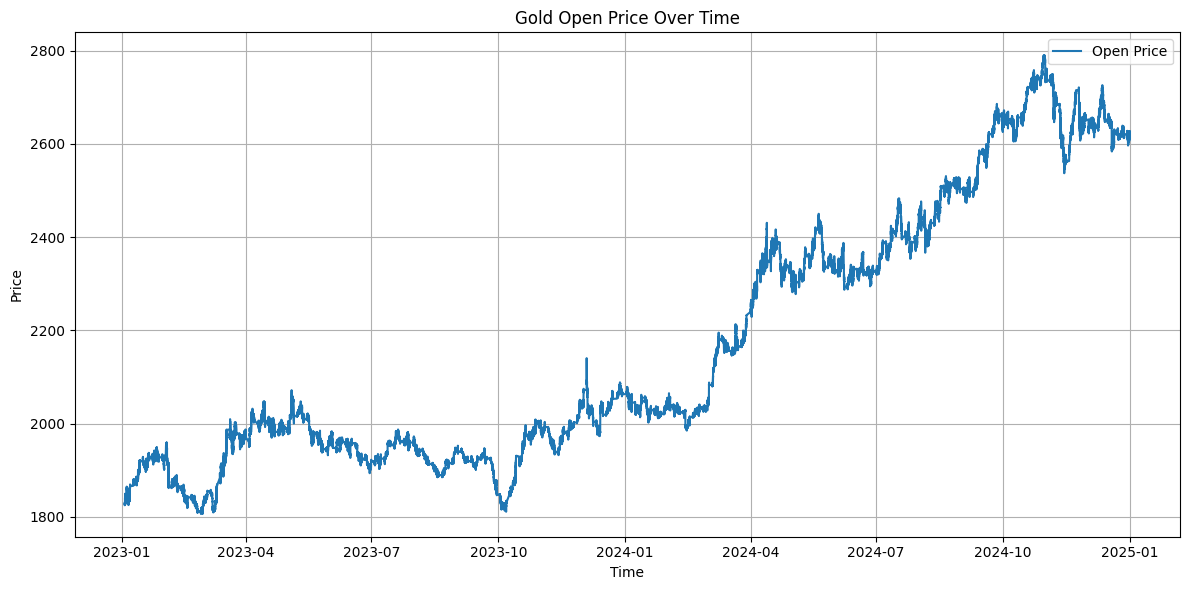
\includegraphics[width=0.8\textwidth]{Figures/Time Series Gold Price.png}
    \caption{Time Series Gold Price}
    \label{fig:time_series_goldprice}
\end{figure}





\newpage

Application of the Kalman filter to a simple state space model, local level model. We assume the hidden state evolves as a random walk and the observations are ... by Gaussian measurement noise. Formally, 

$$x_t = x_{t-1}+q_t, \textbf{ }q_t \sim\mathcal{N}(0, \sigma^2_q),$$
$$y_t = x_t+r_t, \textbf{ } r_t \sim \mathcal{N}(0, \sigma^2_r),$$

with initial prior $x_0 \sim \mathcal{N}(0, P_0)$. Here, $\sigma^2_q$ denotes the state noise variance and $\sigma^2_r$ the measurement noise variance. The state transition and observation matrix reduce to $F=H=1$, which means that the state and measurement equations are scalar. 

By simulating the hidden trajectory $\{x_t\}$ and corresponding noisy observations $\{y_t\}$, we want to illustrate the behavior of the filter. In each iteration the Kalman filter first predicts the next observation and then updates its estimate of the hidden state once the actual measurement becomes available. 

The noise variances $\sigma^2_q$ and $\sigma^2_r$ are unknown and therefore estimated by the maximum likelihood. $\textcolor{orange}{\textbf{needs more explanation}}$



\begin{figure}
    \centering
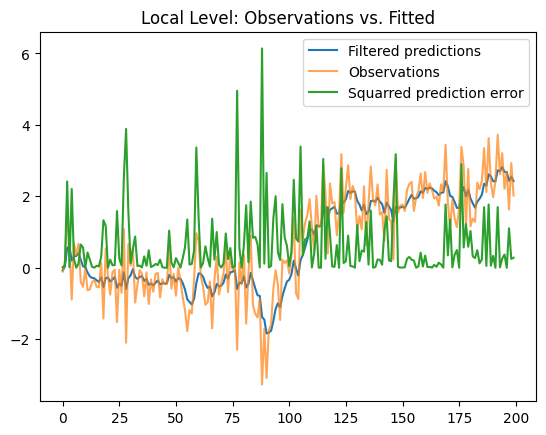
\includegraphics[width=0.5\linewidth]{Figures/Local Level.png}
    \caption{Local Level: Observations vs. Fitted data}
    \label{fig:placeholder}
\end{figure}

Implements a local level (random-walk) state space model with a Kalman filter and then plots fitted vs. observed data.
\begin{enumerate}
    \item simulated a local level time series $x_t$ and noisy observations $y_t$.
    \item defined a one dimensional Kalman filter, where state and measurement are scalar
    \item built energy function of the data 
    \item fitted the process and measurement variances by MLE
    \item computed MSE and plotted results
\end{enumerate}


% CHAPTER 7 APPLICATION OF FINANCIAL TIME SERIES - NOTES
% https://portfoliooptimizationbook.com/

% \cite{palomar:portfolio_optimization}

\section{Prices and Returns}

The price of an asset $p_t$ is the most obvious quantity, where $t$ is the discrete time index, it can also be continuous.

When it comes to modeling, using the logarithm of the prices enhances the mathematical convenience and also represents a wider dynamic range naturally.

% The simplest model for the log-prices is the random walk


\section{Financial Data: I.I.D. Modeling}
EMH: price of security = intrinsic value
any further information about future prospects incorporated in the current price (forecast = current price) 
-> modeling the prices as a random walk $\iff$ returns as a sequence of iid random variables

multiple assets: random variables = return of all assets (multivariate random variable)

under iid: no temporal structure incorporated returns are assumed to be independent distribution of random returns assumed fixed
\section{I.I.D. Model}
ignores temporal structures/ dependency in the data
\[x_t = \mu + \epsilon_t\]
\section{Sample Estimators}
sample mean
sample covariance matrix
estimators are unbiased and consistent
\section{Location Estimators}
\begin{enumerate}
    \item $\textbf{Least square estimator}$
    \item $\textbf{Median estimator}$
    \item $\textbf{Spatial median estimator or geometric median}$
\end{enumerate}

Numerical experiments

For $\textbf{Gaussian data}$, the sample mean is the best estimator (as further analyzed in Section 3.4), the spatial median is almost identical, and the elementwise median is the worst. 
For $\textbf{heavy-tailed data}$, the sample mean is as bad as the median and the spatial median remains the best. 

Overall, the spatial median seems to be the best option as it is robust to outliers and does not underperform under Gaussian data.

\section{Gaussian ML estimators}
Maximum likelihood estimation: important technique in estimation theory
likelihood function

pdf to the iid model, assuming that the residual follows a multivariate normal or Gaussian distribution, is 
\[f(x) = \frac{1}{\sqrt{(2\pi)^N|\Sigma|}}exp(-\frac{1}{2}(x-\mu)^\intercal\Sigma^{-1}(x-\mu))\]


\section{Autoregressive (AR) Model}
% 15. August 2025-------------------------------------------------------

% \textbf{Autoregressive (AR) model}

% \begin{itemize}
%     \item[\textbf{Order 1:}] $$x_t = \varphi_0 + \varphi_1x_{t-1}+\epsilon_t,$$ where $\varphi_0,\varphi_1$ are constants, $\epsilon_t$ we want to be normal distributed with mean 0 and variance $\sigma^2$ since we want to apply the Kalman filter. 
%     The state space model: 
    
%     state: $\begin{bmatrix} 1 \\ x_t
%     \end{bmatrix}$
    
%     transition matrix: $\begin{bmatrix}
%         1 & 0 \\ \varphi_0 & \varphi_1
%     \end{bmatrix}
%     \begin{bmatrix}
%         1 \\ x_t
%     \end{bmatrix} = 
%     \begin{bmatrix}
%         1 \\ \varphi_0 + \varphi_1
%     \end{bmatrix}$

%     covariance matrix: COV = $\begin{bmatrix}
%         0 (\sigma) & 0 \\ 0 & \sigma
%     \end{bmatrix}$
    
%     \item[\textbf{Order n:}] $$x_t= \varphi_0 + \sum_{i=1}^n\varphi_ix_{t-i} + \epsilon_t$$

%     state: $\begin{bmatrix}
%         1 \\ x_t \\ x_{t-1} \\ ... \\ x_{t-n}
%     \end{bmatrix}$

%     transition matrix: $\begin{bmatrix}
%         1 & 0 & ... & 0 & 0 \\
%         \varphi_0 & \varphi_1 & ... & \varphi_{n-1}& \varphi_n \\
%         0 & 1 & 0 & ... & 0 \\
%         0 & ... & ... & ... & 0 \\
%         0 & ... & ... & 0 & 1\\
%     \end{bmatrix}
%     \begin{bmatrix}
%         1 \\ x_t \\ x_{t-1} \\ ... \\ x_{t-n}
%     \end{bmatrix}=
%     \begin{bmatrix}
%         1 \\
%         \varphi_0 + \sum_{i=1}^n\varphi_ix_{t-i} \\
%         x_t\\ 
%         ...\\
%         x_{t-n+1}
%     \end{bmatrix}$
        
%     covariance matrix: $\begin{bmatrix}
%         0 & ... & ... & ... & 0 \\
%         0 & \sigma & 0 & ... & 0 \\
%         0 & ... & ... & ... & 0 \\
%         ... & ... & ... & ... &... \\
%         0 & ... & ... & ... & 0
%     \end{bmatrix}$
% \end{itemize}

%-----------------------------------------------------------------------
AR(1): $x_t = \varphi_0 + \varphi_1 x_{t-1} + \epsilon_t,$ where $\epsilon_t \sim \mathcal{N}(0, \sigma^2)$

\textbf{State vector}
\[
\mathbf x_t =
\begin{bmatrix}
1\\ x_t
\end{bmatrix}.
\]

\textbf{State transition}
\[
\mathbf x_t =
\underbrace{\begin{bmatrix}
1 & 0\\
\varphi_0 & \varphi_1
\end{bmatrix}}_{F}\,
\mathbf x_{t-1}
+
\underbrace{\begin{bmatrix}
0\\ \epsilon_t
\end{bmatrix}}_{\mathbf q_t},
\qquad
\epsilon_t \sim \mathcal N(0,\sigma^2).
\]

\textbf{Process covariance}
\[
Q \;=\;
\begin{bmatrix}
0 & 0\\
0 & \sigma^2
\end{bmatrix}.
\]

\textbf{Measurement equation}
\[
y_t = 
\underbrace{\begin{bmatrix} 0 & 1 \end{bmatrix}}_{H}\,\mathbf x_t + r_t,
\qquad
r_t \sim \mathcal N(0,R).
\]

\textbf{Initialization}
\[
\mathbf x_0 \sim \mathcal N(m_0, P_0).
\]

% AR(p) with intercept in state–space form
\noindent AR(p): $x_t = \varphi_0 + \sum_{i=1}^p \varphi_i x_{t-i} + \epsilon_t,$ where  $\epsilon_t \sim \mathcal{N}(0, \sigma^2)$

\textbf{State vector}
\[
\mathbf{x}_t =
\begin{bmatrix}
1 \\
x_t \\
x_{t-1} \\
\vdots \\
x_{t-p+1}
\end{bmatrix} \in \mathbb{R}^{p+1}.
\]

\textbf{transition matrix:}
\[
F =
\begin{bmatrix}
\varphi_0 & \varphi_1 & \varphi_2 & \cdots & \varphi_p \\
1 & 0 & 0 & \cdots & 0 \\
0 & 1 & 0 & \cdots & 0 \\
0 & 0 & 1 & \cdots & 0 \\
\vdots & \vdots & \vdots & \ddots & \vdots \\
0 & \cdots & 0 & 1 & 0 
\end{bmatrix}
\]

\textbf{observation matrix:}
\[
H =
\begin{bmatrix}
0 & 1 & 0 & \cdots & 0
\end{bmatrix}
\]

\textbf{process noise covariance:}
\[
Q =
\begin{bmatrix}
0 & 0 & \cdots & 0 \\
0 & \sigma^2 & \cdots & 0 \\
\vdots & \vdots & \ddots & \vdots \\
0 & 0 & \cdots & 0
\end{bmatrix}
\in \mathbb{R}^{(p+1)\times(p+1)}.
\]

\textbf{observation equation:}

\[
y_t =
\underbrace{\begin{bmatrix}
0 & 1 & 0 & \cdots & 0
\end{bmatrix}}_{\displaystyle H}
\mathbf{x}_t + r_t,
\qquad
r_t \sim \mathcal{N}(0,R).
\]

\textbf{State transition}
\[
\mathbf{x}_t =
\underbrace{
\begin{bmatrix}
\varphi_0 & \varphi_1 & \varphi_2 & \cdots & \varphi_p \\
1 & 0 & 0 & \cdots & 0 \\
0 & 1 & 0 & \cdots & 0 \\
0 & 0 & 1 & \cdots & 0 \\
\vdots & \vdots & \vdots & \ddots & \vdots \\
0 & 0 & \cdots & 1& 0 
\end{bmatrix}
}_{\displaystyle F}
\mathbf{x}_{t-1}
+
\underbrace{
\begin{bmatrix}
0 \\
\epsilon_t \\
0 \\
\vdots \\
0
\end{bmatrix}
}_{\displaystyle \mathbf{q}_t},
\qquad \epsilon_t \sim \mathcal{N}(0,\sigma^2).
\]



\textbf{Initialization}
Choose prior mean and covariance for the state
\[
\mathbf{x}_0 \sim \mathcal{N}(m_0,\; P_0).
\]


\section*{Markov Property of the AR(p) Model} % ----------------chatGPT----------------

The autoregressive model of order \(p\),
\[
x_t = \varphi_0 + \sum_{i=1}^{p} \varphi_i x_{t-i} + \epsilon_t,
\quad \epsilon_t \sim \mathcal{N}(0, \sigma^2),
\]
is not a first-order Markov process in its scalar form, since the value of \(x_t\) depends on the \(p\) previous values \(x_{t-1}, x_{t-2}, \dots, x_{t-p}\). Therefore, it is a Markov process of order \(p\).

However, when the AR(p) model is written in state-space form, we define a state vector
\[
\mathbf{x}_t =
\begin{bmatrix}
1 \\
x_t \\
x_{t-1} \\
\vdots \\
x_{t-p+1}
\end{bmatrix}
\in \mathbb{R}^{p+1},
\]
and the dynamics become:
\[
\mathbf{x}_t = A \mathbf{x}_{t-1} + \mathbf{w}_t,
\]
where \(\mathbf{w}_t\) is process noise.

In this formulation, the state process \(\{\mathbf{x}_t\}\) satisfies the first-order Markov property:
\[
P(\mathbf{x}_t \mid \mathbf{x}_{t-1}, \mathbf{x}_{t-2}, \dots) = P(\mathbf{x}_t \mid \mathbf{x}_{t-1}).
\]

\textbf{Conclusion:} The scalar AR(p) process is Markov of order \(p\), but its state-space representation defines a first-order Markov process. This Markov structure is essential for the application of the Kalman filter.


% 21. August 2025 ----- Notizen von \cite{palomar:portfolio_optimization}

\section{Financial Data: Time Series Modeling}
\section{Mean Modeling}
- Given past observations we are interested in forecasting the future values of a financial time series
- decide whether to focus on time series of the prices or the returns
- returns tend to be more constant and easier to model 
- prices tend to present a trend 
- Recall: log-prices $y_t=\textbf{log }p_t$ and log-return $x_t= y_t-y_{t-1}$

- the objective is to compute the expectation of the future value of the time series at time $t$ based on the past observations $\mathcal{F}_{t-1}$. This is done in order to uncover potential sturcutral patterns, either through $\mathbb{E}[y_t \mid \mathcal{F}_{t-1}$ for log-prices or $\mathbb{E}[x_t \mid \mathcal{F}_{t-1}$ for log-returns. 


Kapitel 4

% The Kalman filter assumes linear dynamics and Gaussian noises with known variances. The ratio between process noise $\mathbf{Q}$ and measurement noise is important. With very small measurement noise $\mathbf{R}$ the filter can overfit measurements. It overweights the observations and underweights the model dynamics. The filter appears to fit the data perfectly but loses predictive power because it treats random observation noise as real signal. While with very small process noise $\mathbf{Q}$ the filter may be too \textcolor{orange}{find correct word}. The filter becomes overconfident in its model dynamics and underweights new measurements. The estimated states change only slowly and may lag behind the true process. Especially when the underlying system evolves faster than expected. % Intuitive it means that the filter trusts its model too much and ignores the measurements. The state estimate reacts slowly to new data. % for the example, if Q is large, the filter assumes the object can move unpredictably; it follows the data closely, if Q is very small the filter assumes smooth movements; it barely updates when the object suddendly turns. This behaviour shows the importance of correctly identifying ratio between process and measurement noise variances. 

% --------------------------------------------------------------------------------------------------------------------------------------------------------------------------------------------

% what is a Kalman Filter and its meaning, applications, why relevant in my thesis; mathematical background, state space representation, Gaussian noise assumptions, recursive Bayesian estimation (predict-update cycle), introduce predition and update step, covariance matrices




% Google Colab - Filter Random Walk
\section*{Random Walk Model}
% \cite{sarkka:bayesian_filtering}

\noindent   
\textbf{State transition equation:}
\[x_t= x_{t-1} + q_{t-1}, \quad q_t \sim \mathcal{N}(0,Q)\]

\medskip
\noindent   
\textbf{Observation equation:}
$$y_t = x_t+ r_t, \quad r_t \sim \mathcal{N}(0,R)$$ 

$x_t$ is the hidden state and $y_t$ is the measurement with state transition matrix $F=1$, observation matrix $H=1$, process noise covariance $Q$ and observation noise covariance $R$.

The random walk model is one of the simplest state space models. The model assumes that the hidden state evolves over time and the observations are noisy measurements of this state. In this model, the expected state at time $t$ given the previous state is simply the same as the previous state\cmmnt{, $\mathbb{E}[x_t |x_{t-1}]=x_{t-1}$}. The model therefore describes a process with no deterministic dynamics, only random fluctuations. 

In the code $\cmmnt{Train and Test on RandomWalk.ipynb}$, the model parameters are estimated using the training dataset. The process noise variance $Q$ and and observation noise variance $R$ are fitted to maximize the likelihood of the observed data under the Kalman filter. The Kalman filter is then used to compute the filtered state means and covariances for each time step. 
An important observation from the fitted parameters is that the estimated observation noise variance $R$ is very small \cmmnt{indicating high confidence in measurements}. The model is therefore flexible enough to closely follow the observed data. 
As a consequence, the filtered estimates lie almost exactly on top of the observed values. % if we believe observation is noise free then the best estimate of the true state after seeing y_t is simply x_t


\medskip
\noindent
\textit{Formal prediction to be added!}

The predictions of the random walk are given by $\hat x_{t+1|t} = \mathbb{E}[x_{t+1|y_{1:t}}]$. Since the expected increment is zero, the predicted mean for the next state is equal to the most recent filtered estimate. This means that the distribution $p(x_{t+1}|y_{1:t})$ is centered at the current state

% Google Colab - Train and Test Filter Random Walk

\begin{figure}[H]
    \centering
    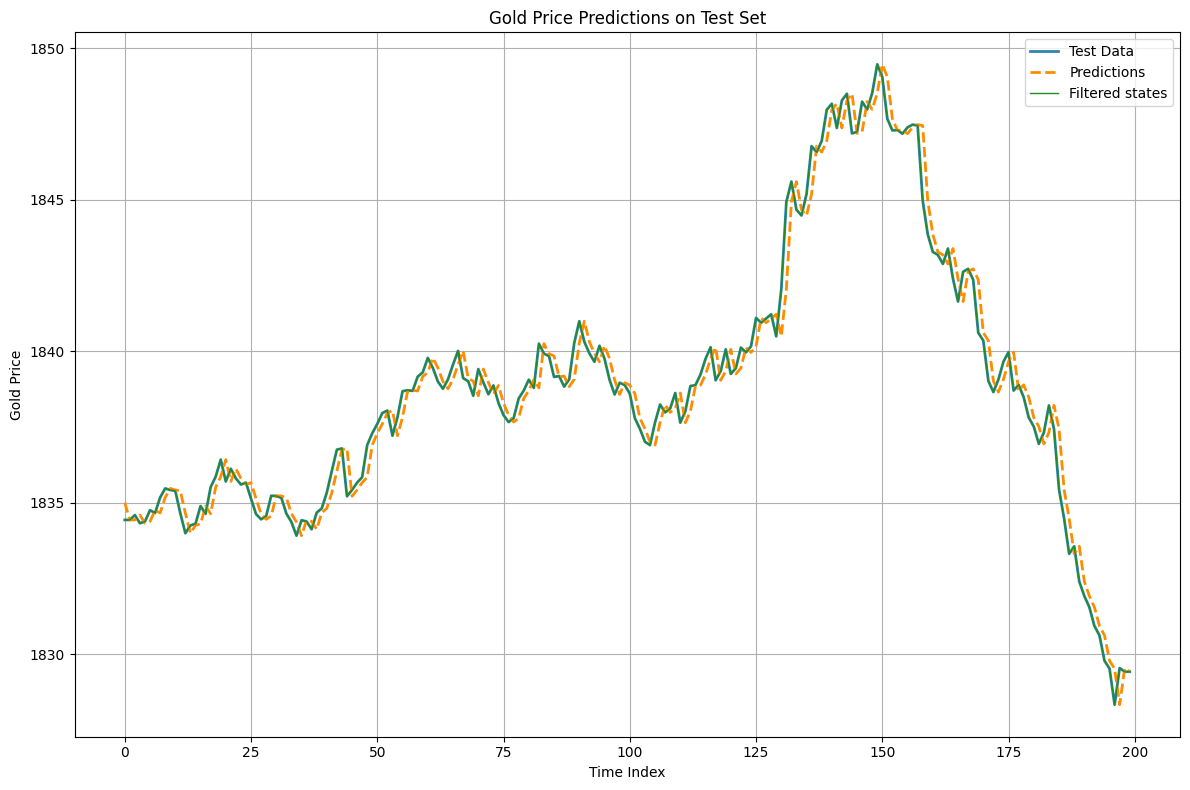
\includegraphics[width=0.5\linewidth]{Figures/Gold Price Predictions Random Walk.png}
    \caption{Gold price predictions on test set with random walk}
    \label{fig:randwal}
\end{figure}

In Figure \ref{fig:randwal}, we observe that the filtered states follow the observations almost same. This is expected because the estimated observation noise is very small. On the other hand, the predicted values are slightly shifted from the true observations because the model uses the current filtered estimate as its best guess for the next state. 

The predictions would appear more random if the process noise covariance $Q$ were increased. \cmmnt{Filtering estimates the state given the current observation after having seen it so it can almost exactly match the observed data when $R$ is small. Prediction estimates the state for the next time step before seeing the observation, so it cannot adjust to new data and reflects only the model's prior dynamics.}




\newpage
%  Linear Growth Model/ Local Linear Trend State Space Model 
% \cite{triantafyllopoulos:bayesian_state_space}
\section*{Local Linear Trend Model}

\medskip
\noindent 
\textbf{State vector:}
\[x_t= \begin{bmatrix} 
                \ell_t \\ 
                \mu_t 
            \end{bmatrix}\]

where $\ell_t$ is the local level and $\mu_t$ is the local slope.

\medskip
\noindent
\textbf{State transition equation:}
$$x_{t+1} = Fx_t + q_t$$ 

with transition matrix
$F=\begin{bmatrix} 
        1 & 1 \\ 
        0 & 1
    \end{bmatrix},$
$q_t = \begin{bmatrix}
    \eta_t \\ \zeta_t
\end{bmatrix}$
and process noise covariance
$Q=\begin{bmatrix} 
        \sigma^2_\eta & 0 \\ 
        0 & \sigma^2_\zeta 
    \end{bmatrix}.$

\medskip
\noindent     
\textbf{Observation equation:}
\[
y_t = Hx_t+\epsilon_t, \quad \epsilon_t \sim \mathcal{N}(0, \sigma^2_\epsilon)
\]
with the observation matrix \[H=\begin{bmatrix} 1 & 0 \end{bmatrix}.\]
\begin{itemize}
    \item $\eta_t$ level noise, 
    \item $\zeta_t$ slope noise and
    \item $\epsilon_t$ observation noise. 
    \item $\mu_t$ follows a linear function and a random error $\zeta_t$
\end{itemize}

\medskip
\noindent 
\textbf{Component form:}
% component form shows the individual dynamics of y_t and \beta_t whereas matrix form is compact and convenient for algorithms (Kalman filter, smoothing)
\begin{align*}
    % level: previous level + slope + random noise \eta_t
    \ell_{t+1} &= \ell_t + \mu_t + \eta_t, &\eta_t \sim \mathcal{N}(0, \sigma^2_\eta)\\
    % slope: random walk + noise \zeta_t
    \mu_{t+1} &= \mu_t + \zeta_t, &\zeta_t \sim \mathcal{N}(0, \sigma^2_\zeta)\\
    % observation equation 
    y_t &= \ell_t+\epsilon_t, &\epsilon_t \sim \mathcal{N}(0, \sigma^2_\epsilon)
\end{align*}


\medskip
The local linear trend model is an extension of the random walk that introduces a trend component to capture local slopes \cmmnt{or drifts} in the data over time. The state vector consists of two elements, the local level $\ell_t$ and the local slope $\mu_t$. $Q$ is the process noise covariance for the level and trend components. While the random walk assumes that the expected change of the state is zero, the local linear trend model allows for a time-varying mean change determined by $\mu_t$. Again, in the code \cmmnt{Train and Test von FilterLocalLinearTrendModel.ipynb}, the model parameters are estimated using the training dataset. The process and observation noise variances are fitted by maximizing the likelihood under the Kalman filter. The filter then computes the filtered state means and covariances at each time step. The filtered level follows the data closely, while the estimated trend captures the local direction of the change. 

\medskip
\noindent
\textit{Formal prediction to be added!}


\begin{figure}[H]
    \centering
    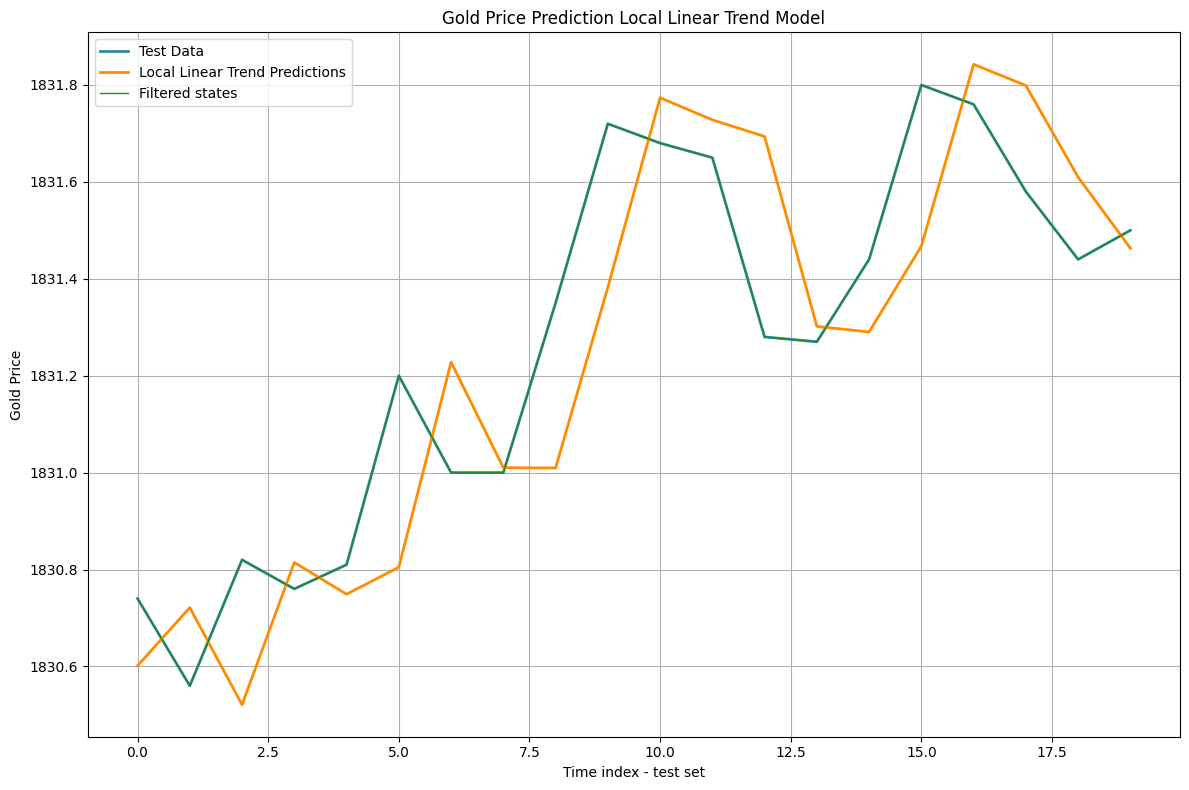
\includegraphics[width=0.5\linewidth]{Figures/Gold Price Predictions Local Linear Trend Model.png}
    \caption{Gold price predictions on test Set with local linear trend model}
    \label{fig:loclin}
\end{figure}

In Figure \ref{fig:loclin}, we again observe that the filtered state follows the observation in a nearly identical manner. This is also expected because the estimated observation noise is very small. However, the predicted values are slightly shifted relative to the observations because the model uses the current filtered estimate as its best guess for the next state. 

If the process noise covariance $Q$ were increased, the prediction would appear more random. 


% -----------------------------------------------------------
% Color Scheme:
% 1. Actual Data: '#2E86AB' 
% 2. Predictions: 'darkorange' 
% 3. Filtered States: 'forestgreen' 
% 4. Prediction Errors: 'purple' 
% 5. Filtered Errors: 'red' 
% 6. Zero Line: 'gray' 

% Consistent Sizing:
% 1.  All figures use $FIG_SIZE = (12, 8)$ for uniformity

% Enhanced Analysis:
% - Shows both prediction errors AND filtered state errors
% - Comprehensive performance metrics
% - Clear distinction between different types of estimates


Probability 

% Let $\mathbf{x} \in \mathbb{R}^n$ be a Gaussian random vector
% \[
% \mathbf{x} \sim \mathcal{N}(\mathbf{m}, \mathbf{P}),
% \]
% and consider a linear transformation
% \[
% \mathbf{y} := \mathbf{A}\mathbf{x} + \mathbf{b},
% \]
% where $\mathbf{A} \in \mathbb{R}^{m \times n}$ is a deterministic matrix and $\mathbf{b} \in \mathbb{R}^{m}$ is a constant vector. In this case the transformed variable $\mathbf{y}$ is also Gaussian. 
% %
% The mean of $\mathbf{y}$ is obtained using linearity of expectation:
% \begin{align*}
% \mathbb{E}[\mathbf{y}]
% &=\mathbb{E}[\mathbf{A}\mathbf{x} + \mathbf{b}] \\
% &=\mathbf{A}\mathbb{E}[\mathbf{x}] + \mathbf{b} \\
% &=\mathbf{A}\mathbf{m} + \mathbf{b}.
% \end{align*}
% The covariance of $\mathbf{y}$ follows from the covariance identity
% $\mathrm{Cov}(\mathbf{A}\mathbf{x}) = \mathbf{A}\,\mathrm{Cov}(\mathbf{x})\,\mathbf{A}^\top$:
% \begin{align*}  
% \mathrm{Cov}(\mathbf{y})
% &= \mathrm{Cov}(\mathbf{A}\mathbf{x}) \\
% &= \mathbf{A}\mathbf{P}\mathbf{A}^\top.
% \end{align*}
% Therefore the transformed variable $\mathbf{y}$ follows the Gaussian distribution
% \begin{equation}
% \label{affine transformation}
% \mathbf{y} \sim
% \mathcal{N}(\mathbf{A}\mathbf{m} + \mathbf{b},\; \mathbf{A}\mathbf{P}\mathbf{A}^\top).
% \end{equation}

%This property is particularly useful in dynamical systems, where the state of a system evolves through linear transformations. In such models, Gaussian uncertainty remains Gaussian after each transformation, which makes recursive estimation algorithms such as the Kalman filter computationally tractable. \cite[Ch.~3]{murphy:probabilistic_ml_introduction}

% In the Kalman filter, each prediction is an affine transformation of the previous Gaussian belief, ensuring that the resulting distribution remains Gaussian. In the special case where the covariance matrix $\mathbf{P}=0$, the Gaussian distribution collapses to a single point at $\boldsymbol{\mu}$, meaning there is no uncertainty in the variable. 


\section{Exact solutions in Bayesian filtering}\label{sec: exact solutions in bayesian filtering}
% \st{In theory, Bayesian filtering works for any state space model. But in practice, we usually can't compute the exact posterior distribution because the required integrals are too difficult or do not have closed-form solutions. Exact solutions to the Bayesian filtering problem are only possible under restrictive conditions. 

% The conditions: }
% \begin{itemize} 
%     \item \textbf{Linear system}: transition and measurement are linear in the state. 
%     \item \textbf{Gaussian noise}: process and measurement noise are normally distributed. 
% \end{itemize}
% When the system is linear and the noise is Gaussian, the exact solution is provided by the Kalman filter. When the system is discrete, it is called a hidden Markov model and can be solved using matrix algebra, provided the state space is not too large.

% \st{Under these conditions the filtering equations lead to closed-form solutions.}
%Under these assumptions, the Bayesian filtering equations simplify to closed-form expressions.

% The next chapter will show the explicit equations of the Kalman filter and how they are applied to this drone model.

Kapitel 4.4
% The Kalman filter is important because it is used to estimate and predict hidden states in time series models. The data can be noisy and the filter helps to combine the information from the model and the observations in a optimal way. It's useful for studying financial and economic data, where we want to follow smooth trends and understand uncertainty in the predictions \cite{palomar:portfolio_optimization}. However it works under two main assumptions. That the system is linear and the noise is Gaussian. These assumptions make the filter easy to use but it also comes with limitations. If the system behaves in a non-linear way or if the noise is not Gaussian, the filter doesn't work. 
% To handle such cases there are extension like Extended Kalman Filter (EKF) and the Unscented Kalman Filter (UKF). These methods follow the same idea but can deal better with non-linear models \cite[Ch. X]{sarkka:bayesian_filtering}.
